\documentclass[ngerman,11pt]{article}

\usepackage[left=2.5cm, right=2.5cm, top=2cm, bottom=2cm]{geometry}
\usepackage{babel}
\usepackage{listings}
\usepackage{color}
\usepackage{hyperref}
\usepackage{csquotes}
\usepackage{awesomebox}
\MakeOuterQuote{"}

\pagenumbering{gobble}
\renewcommand{\lstlistingname}{Schnipsel}

% see overleaf
\definecolor{lightgray}{rgb}{0.95, 0.95, 0.95}
\definecolor{darkgray}{rgb}{0.4, 0.4, 0.4}
%\definecolor{purple}{rgb}{0.65, 0.12, 0.82}
\definecolor{editorGray}{rgb}{0.95, 0.95, 0.95}
\definecolor{editorOcher}{rgb}{1, 0.5, 0} % #FF7F00 -> rgb(239, 169, 0)
\definecolor{editorGreen}{rgb}{0, 0.5, 0} % #007C00 -> rgb(0, 124, 0)
\definecolor{orange}{rgb}{1,0.45,0.13}
\definecolor{olive}{rgb}{0.17,0.59,0.20}
\definecolor{brown}{rgb}{0.69,0.31,0.31}
\definecolor{purple}{rgb}{0.38,0.18,0.81}
\definecolor{lightblue}{rgb}{0.1,0.57,0.7}
\definecolor{lightred}{rgb}{1,0.4,0.5}

\definecolor{dkgreen}{rgb}{0,0.6,0}
\definecolor{gray}{rgb}{0.5,0.5,0.5}
\definecolor{mauve}{rgb}{0.58,0,0.82}

\lstdefinelanguage{CSS}{
    keywords={color,background-image:,margin,padding,font,weight,display,position,top,left,right,bottom,list,style,border,size,white,space,min,width, transition:, transform:, transition-property, transition-duration, transition-timing-function},
    sensitive=true,
    morecomment=[l]{//},
    morecomment=[s]{/*}{*/},
    morestring=[b]',
    morestring=[b]",
    alsoletter={:},
    alsodigit={-}
}

% JavaScript
\lstdefinelanguage{JavaScript}{
    morekeywords={typeof, new, true, false, catch, function, return, null, catch, switch, var, if, in, while, do, else, case, break},
    morecomment=[s]{/*}{*/},
    morecomment=[l]//,
    morestring=[b]",
    morestring=[b]'
}

\lstdefinelanguage{HTML5}{
    language=html,
    sensitive=true,
    alsoletter={<>=-},
    morecomment=[s]{<!-}{-->},
    tag=[s],
    otherkeywords={
        % General
        >,
        % Standard tags
        <!DOCTYPE,
        </html, <html, <head, <title, </title, <style, </style, <link, </head, <meta, />,
        % headings
        </h1, <h1, </h2, <h2, </ul, <ul, </ol, <ol, </li, <li, <img, </a, <a,
        % body
        </body, <body,
        % Divs
        </div, <div, </div>,
        % Paragraphs
        </p, <p, </p>,
        % scripts
        </script, <script,
        % More tags...
        <canvas, /canvas>, <svg, <rect, <animateTransform, </rect>, </svg>, <video, <source, <iframe, </iframe>, </video>, <image, </image>, <header, </header, <article, </article
    },
    ndkeywords={
        % General
        =,
        % HTML attributes
        charset=, src=, id=, width=, height=, style=, type=, rel=, href=,
        % SVG attributes
        fill=, attributeName=, begin=, dur=, from=, to=, poster=, controls=, x=, y=, repeatCount=, xlink:href=,
        % properties
        margin:, padding:, background-image:, border:, top:, left:, position:, width:, height:, margin-top:, margin-bottom:, font-size:, line-height:,
        % CSS3 properties
        transform:, -moz-transform:, -webkit-transform:,
        animation:, -webkit-animation:,
        transition:,  transition-duration:, transition-property:, transition-timing-function:,
    }
}

\lstdefinestyle{htmlcssjs} {%
% General design
%  backgroundcolor=\color{editorGray},
    basicstyle={\footnotesize\ttfamily},
    frame=b,
% line-numbers
    xleftmargin={0.75cm},
    numbers=left,
    stepnumber=1,
    firstnumber=1,
    numberfirstline=true,
% Code design
    identifierstyle=\color{black},
    keywordstyle=\color{blue}\bfseries,
    ndkeywordstyle=\color{editorGreen}\bfseries,
    stringstyle=\color{editorOcher}\ttfamily,
    commentstyle=\color{brown}\ttfamily,
% Code
    language=HTML5,
    alsolanguage=CSS,
    alsodigit={.:;},
    tabsize=2,
    showtabs=false,
    showspaces=false,
    showstringspaces=false,
    extendedchars=true,
    breaklines=true,
% German umlauts
    literate=%
        {Ö}{{\"O}}1
        {Ä}{{\"A}}1
        {Ü}{{\"U}}1
        {ß}{{\ss}}1
        {ü}{{\"u}}1
        {ä}{{\"a}}1
        {ö}{{\"o}}1
}

\lstset{frame=tb,
    language=Java,
    aboveskip=3mm,
    belowskip=3mm,
    showstringspaces=false,
    captionpos=b,
    columns=flexible,
    basicstyle={\small\ttfamily},
    numbers=left,
    numberstyle=\tiny\color{gray},
    keywordstyle=\color{blue},
    commentstyle=\color{dkgreen},
    commentstyle=\color{dkgreen},
    stringstyle=\color{mauve},
    breaklines=true,
    breakatwhitespace=true,
    tabsize=3,
    inputencoding=utf8
}

% Packages
\usepackage{amsmath}
\usepackage{graphicx}

% Document
\setlength{\parindent}{0pt}
\begin{document}

{\huge \textbf{Einführung in Flexbox}}
    \\

    Mit dem \textit{Layout} bezeichnet man die \textit{Anordnung} der Elemente.
    Das Layout beeinflusst die "Bedienbarkeit" (\textit{User Experience}) und das Erscheinungsbild einer Website. \\

    Beispiel:

    \begin{center}
        
\includegraphics[width=0.7\textwidth]{aachener_zeitung_pc}
        \footnote{Quelle: \url{https://www.aachener-zeitung.de}}
    \end{center}

    Dies ist die Website der Aachener Zeitung (Stand 22.\ Januar 2025).
    Was für ein Layout erkennen wir?

    \begin{center}
        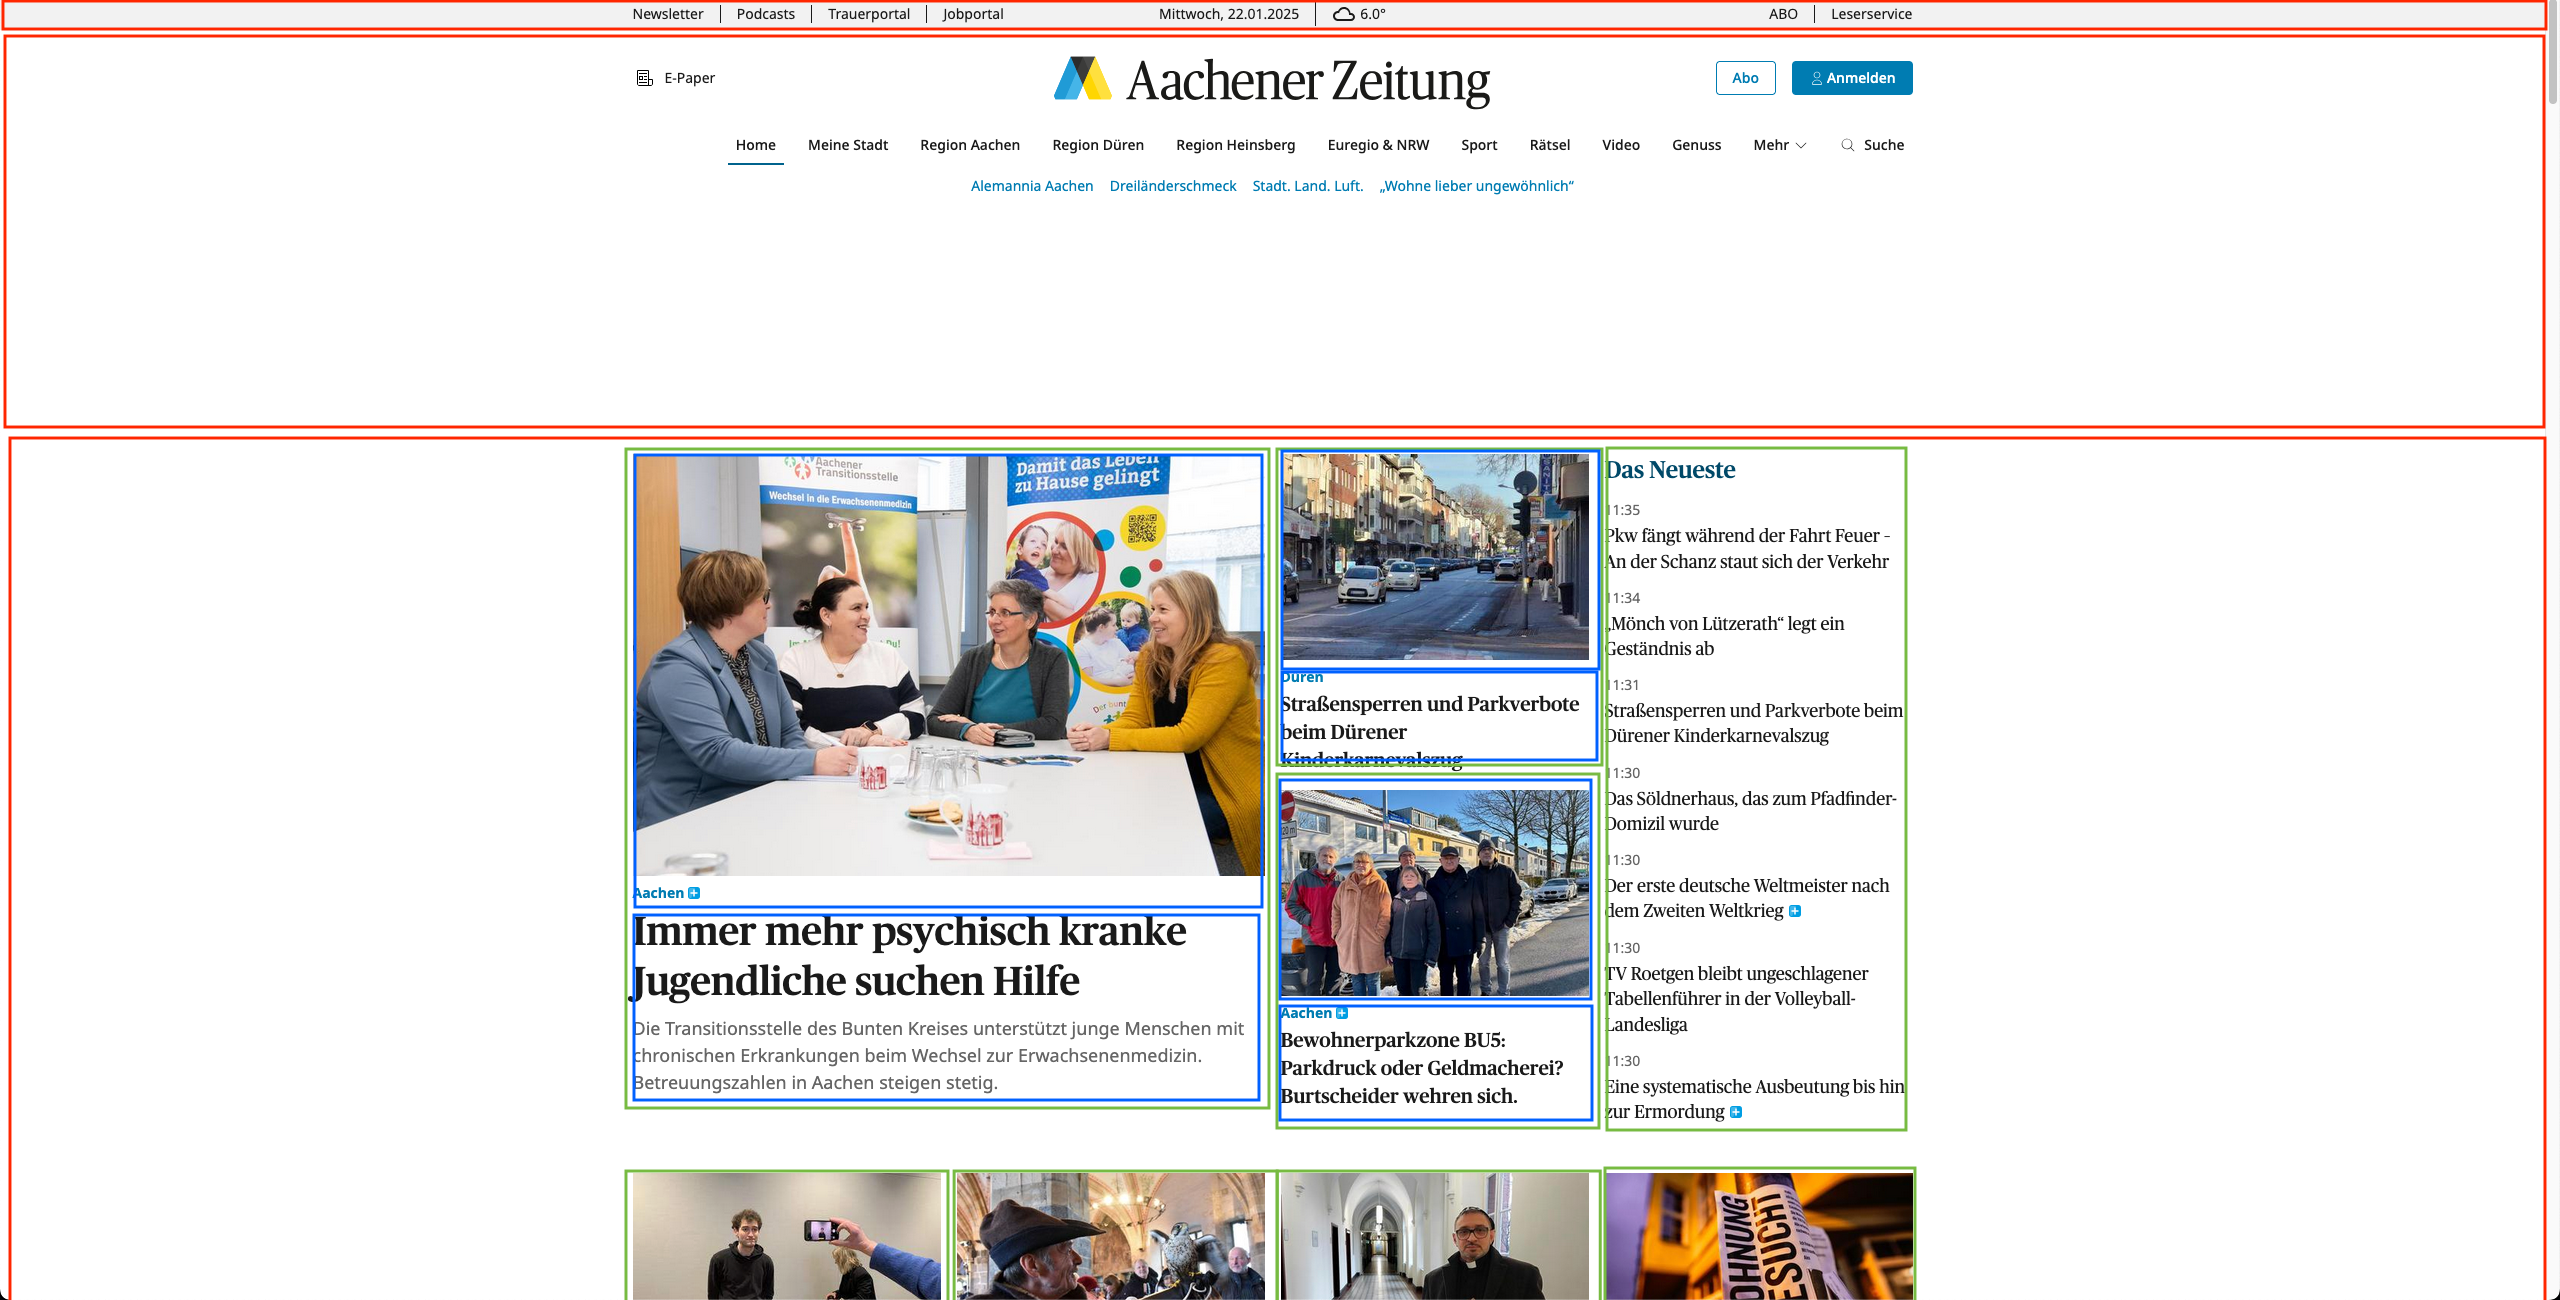
\includegraphics[width=0.7\textwidth]{aachener_zeitung_lined}
        \footnote{Quelle: \url{https://www.aachener-zeitung.de}}
    \end{center}

    Auf der gröbsten Ebene ist die Seite unterteilt in 3 Abschnitte, die untereinander angeordnet sind:
    Die Kopfleiste (Header), Der Titel- /Menüabschnitt und der große Abschnitt für die Artikelübersicht (rote Linien).
    Schauen wir uns die Artikelübersicht näher an, können wir weitere Unterteilungen und Anordnungen finden:
    Die Artikel selbst sind in unterschiedlich großen Kacheln in einer Art Raster angeordnet (Grüne Linien),
    Überschriften und Bilder jeweils untereinander (blaue Texte).

    \notebox{
        Öffnen wir die Seite auf dem Handy, stellen wir fest, dass das Layout ein völlig anderes ist.
        Heutzutage werden Websiten von den unterschiedlichsten Geräten aus verwendet (PC, Laptops, Smartphone,
        faltbares Smartphone, Smartwatch, Smart-TV, \dots) und als Entwickler will man sicherstellen, dass
        möglichst vielen Nutzern eine vernünftige Darstellung geboten wird.
    }

    Um das Layout einer Website zu definieren, gibt es verschiedene Möglichkeiten.
    Das erste Layout-Werkzeug was wir betrachten wollen ist \textit{Flexbox}.
    Bevor wir das tun, wollen wir uns noch eine Möglichkeit ansehen, wie man mit CSS weniger umständlich arbeiten kann.

    \section{Ausgelagertes CSS}

    Wir haben bisher \textit{Inline-CSS} verwendet, das heißt, unsere CSS Eigenschaften samt ihrer Werte direkt an die HTML
    Elemente drangeschrieben, was wie folgt aussieht:

    \begin{lstlisting}[type=htmlcssjs]
<h1 style="font-size: 100pt">Ein riiiiesengrosser Text..</h1>
    \end{lstlisting}

    Wenn wir viele verschiedene CSS Regeln haben und sich gleiche Regeln für verschiedene Elemente
    wiederholen, wird es irgendwann sehr unübersichtlich:

    \begin{lstlisting}[type=htmlcssjs]
<h3 style="font-size: 16pt; text-shadow: black 1px 1px 3px;">Irgendeine Ueberschrift</h3>
<h3 style="font-size: 16pt; text-shadow: black 1px 1px 3px;">Was anderes..</h3>
<h3 style="font-size: 16pt; text-shadow: black 1px 1px 3px;">Sonst was...</h3>
<h3 style="font-size: 16pt; text-shadow: black 1px 1px 3px;">Und nochmal...</h3>
<h3 style="font-size: 16pt; text-shadow: black 1px 1px 3px;">und nochmal...</h3>
<h3 style="font-size: 16pt; text-shadow: black 1px 1px 3px;">puh...</h3>
    \end{lstlisting}

    Was wir tun können, ist das CSS \textit{auszulagern}.
    Das funktioniert wie folgt:

    \begin{lstlisting}[type=htmlcssjs]
<!doctype html>
<html>
    <head>
        <style>
            .mein-text {
                font-size: 16pt;
                text-shadow: black 1px 1px 3px;
                color: green;
                ...
            }
        </style>
    </head>
    <body>
        <h3 class="mein-text">Text...</h3>
        <h3 class="mein-text">Mehr Text...</h3>
        <h3 class="mein-text">Text...</h3>
        <h3 class="mein-text">Mehr Text...</h3>
    </body>
</html>
    \end{lstlisting}

    Wie funktioniert das?
    Neu ist das attribut \textit{class} (Klasse).
    Mit Klassen können wir verschiedene CSS-Regeln unter einem Namen gruppieren.
    Im Beispiel oben gruppieren wir die Angaben für \lstinline{font-size}, \lstinline{text-shadow} und \lstinline{color}
    und nennen die Klasse \lstinline{mein-text}.
    Diese Klasse können wir dann einem Element mithilfe des \textit{class} Attributs zuweisen, indem wir schreiben

    \begin{lstlisting}[type=htmlcssjs]
<element class="mein-text">...</element>
    \end{lstlisting}

    \warningbox{Beachte genau die Notation. Die CSS Regeln gehören in das {\verb(<style>} Element,
        dieses wiederum in den {\verb(<head>}.
        Die Regeln für eine Klasse kommen in geschweifte Klammern, und im style tag steht vor dem
        Klassenname ein ".". Die CSS Regeln werden mit Semikolons getrennt.
    }

    Wir können einem Element auch mehrere Klassen zuweisen, indem wir diese einfach mit einem Leerzeichen trennen. \\

    Beispiel:

    \begin{lstlisting}[type=htmlcssjs]
<!doctype html>
<html>
    <head>
        <style>
            .text-gross {
                font-size: 30pt;
            }

            .text-blau {
                color: blue;
            }
        </style>
    </head>
    <body>
        <h1 class="text-gross text-blau">
            Dieser Text wird sowohl gross als auch blau erscheinen.
        </h1>
    </body>
</html>
    \end{lstlisting}

\end{document}
